\begin{frame}
  \frametitle{Images as arrays}

  \begin{center}
    Grayscale images $\leftrightarrow$ 2-d arrays of $M \times N$ pixel intensities
    \vskip20pt
    \only<1>{
\includegraphics[height=0.5\textheight]{../../code/image_data/sample_digit.png}}
    \only<2>{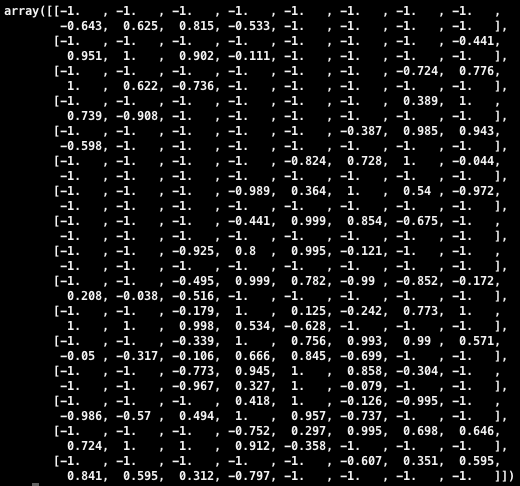
\includegraphics[height=0.5\textheight]{image_array.png}}
  \end{center}

\end{frame}

\begin{frame}[fragile]
  \frametitle{Images as arrays}

  \begin{center}
    Color images $\leftrightarrow$ 3-d arrays of $M \times N \times 3$ RGB pixel intensities
    \vskip20pt
    \only<1>{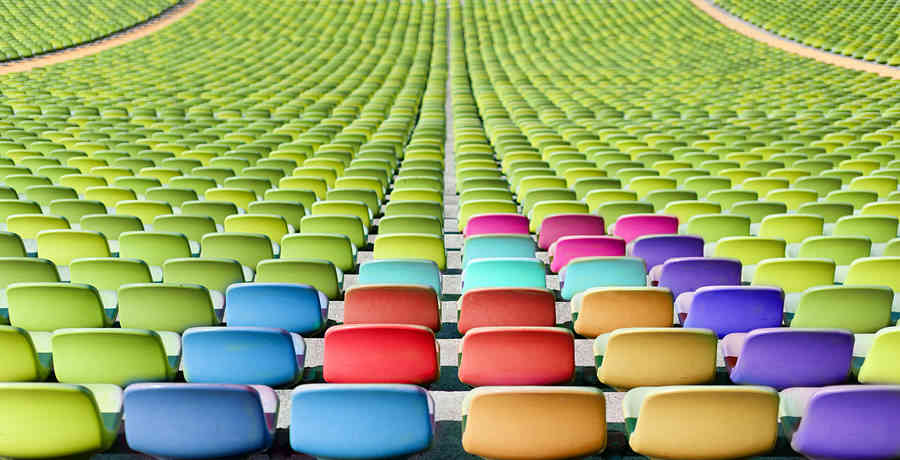
\includegraphics[height=0.45\textwidth]{../../code/image_data/chairs.jpg}}
    \only<2>{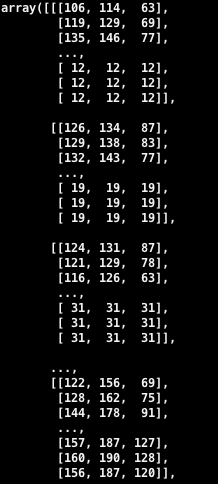
\includegraphics[height=0.5\textheight]{image_array_color.png}}
  \end{center}

    \begin{block}{}
        \begin{lstlisting}[language=python]
import matplotlib.image as mpimg
I = mpimg.imread('chairs.jpg')
        \end{lstlisting}
    \end{block}

\end{frame}

% jntj: bag of pixels, intensity histogram, spatial features

\begin{frame}
  \frametitle{Intensity histograms}

  \begin{center}
    Disregard all spatial information, simply count pixels by intensities \\
    (e.g. lots of bright green and dark blue pixels)
    \vskip20pt
  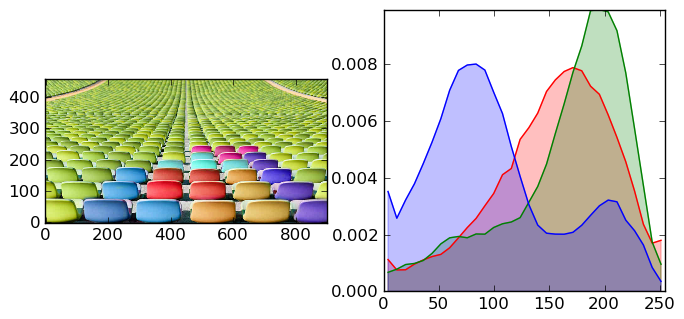
\includegraphics[width=\textwidth]{../../code/image_data/chairs_32.png}
  \end{center}

\end{frame}


\begin{frame}
  \frametitle{Intensity histograms}

  \begin{center}
    How many bins for pixel intensities?
    \vskip20pt
    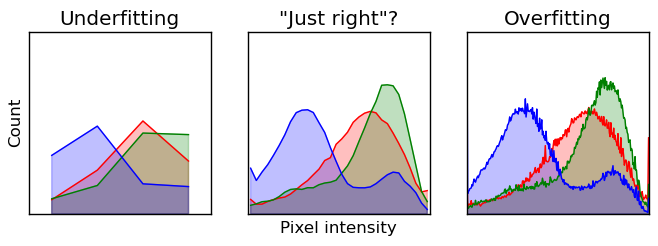
\includegraphics[width=0.75\textwidth]{chairs_hists.png}
    \vskip20pt
    \textbf{Too many} bins gives a noisy, \textbf{overly complex} representation of the data,\\
    while using \textbf{too few} bins results in an \textbf{overly simple} one
  \end{center}

\end{frame}

